\section{Language Models}

\begin{frame}[c]{Basic Terminology}
    \large
    \begin{itemize}[<+(1)->]
        \item   \textbf{Token:} String of arbitrary length, usually 3-4 characters
            \begin{itemize}
                \item Refer to my previous talk about the transformer architecture for more details on internals
            \end{itemize}
        \item   \textbf{Context Length:} Amount of tokens a model can process concurrently as input
        \item   \textbf{Single-shot / Multi-shot:} Evaluation setting in which a \gls{LLM} is being provided with one or multiple examples of the task to fulfill
        \item   \textbf{Zero-shot:} Evaluation setting in which no task examples are provided
    \end{itemize}
\end{frame}


\begin{frame}[c]{The Transformer Architecture}
    \begin{figure}
        \captionsetup[subfigure]{labelformat=empty}
        \begin{subfigure}{0.3\textwidth}
            \centering
            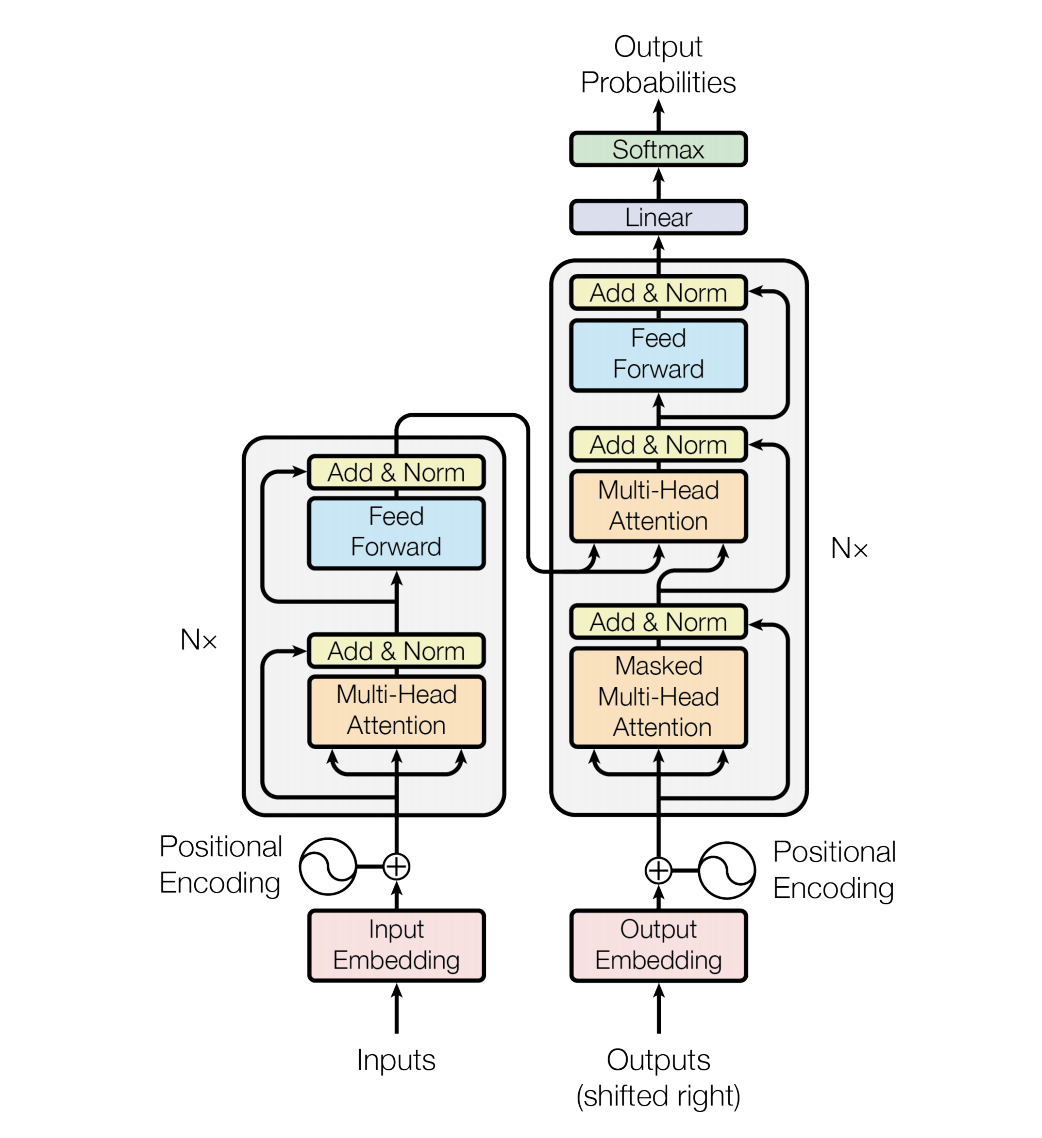
\includegraphics[height=0.6\textheight]{transformer}
            \caption{
                Original Transformer Architecture \\
            Image Source: \cite{vaswani_attention_2017}
            } 
        \end{subfigure}%
        \begin{subfigure}{0.45\textwidth}
            Most Prominent Changes:
            \begin{itemize}[<+(1)->]
                \item Activation Function: \gls{SwiGLU} \cite{shazeer_glu_2020} instead of \gls{ReLU}
                \item Positional Encoding: \gls{RoPE} \cite{su_roformer_2022}, and \textit{on each layer}
                \item Normalization with RMSNorm \cite{ba_layer_2016} \textit{before} instead of after each layer
                \item Attention: Often a variant of Sparse Attention \cite{child_generating_2019} or FlashAttention \cite{dao_flashattention_2022}
                \item Most Recently: The usage of \acrfull{GQA} \cite{ainslie_gqa_2023}
            \end{itemize}
            \vspace{1em}
        \end{subfigure}%
        \hspace{1em}
        \begin{subfigure}{0.2\textwidth}
            \centering
            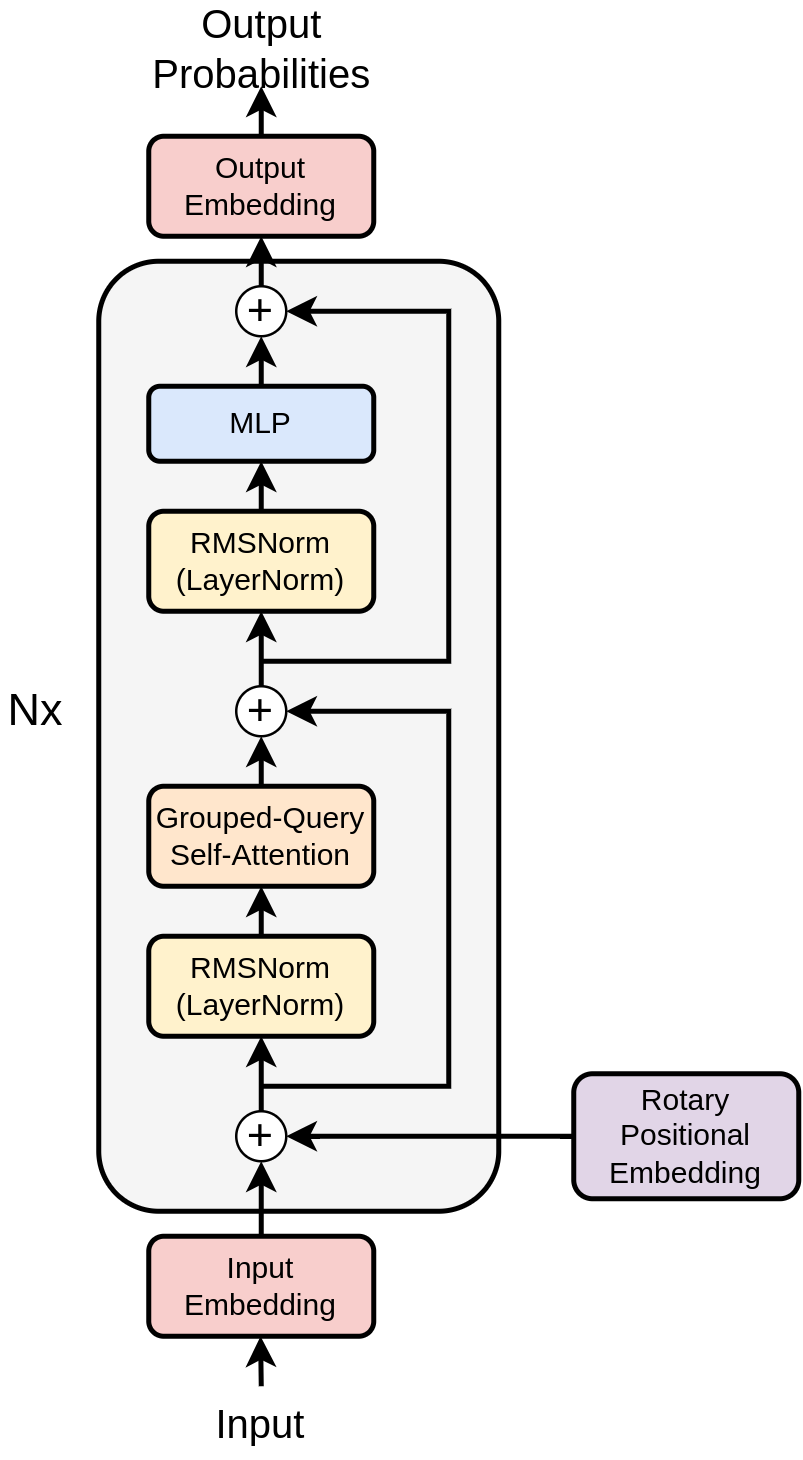
\includegraphics[height=0.6\textheight]{modern_transformer}
            \caption{
                Modern Transformer Architecture
            }
        \end{subfigure}
    \end{figure} 
\end{frame}


\begin{frame}[c]{Large Language Model Parameter Count}
    \centering
    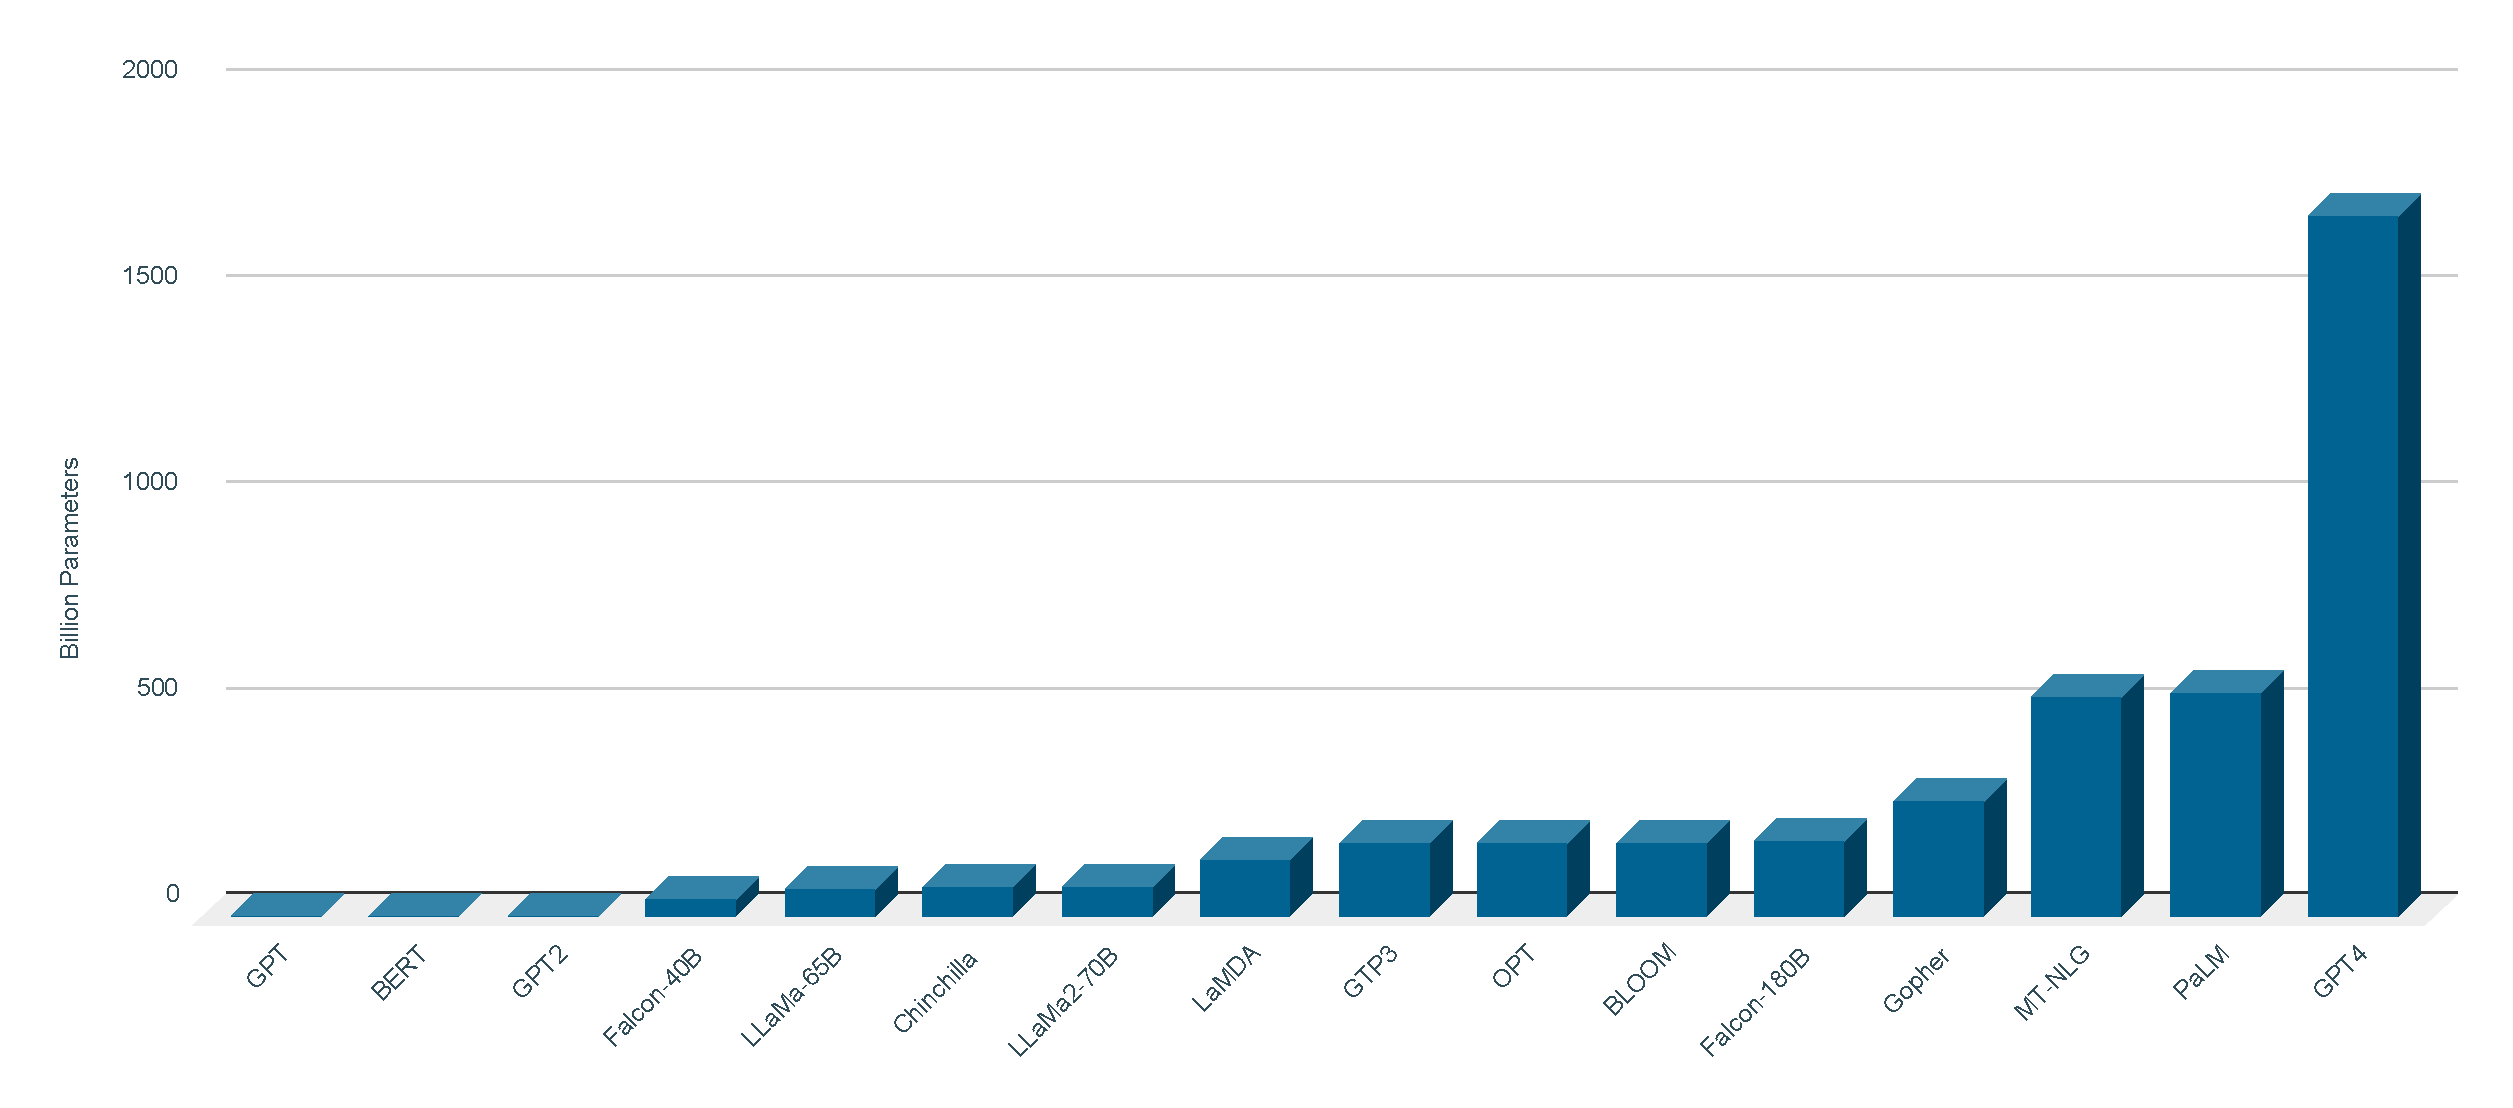
\includegraphics[height=0.7\textheight]{comparison_absolute}
\end{frame}

\begin{frame}[c]{Large Language Model Parameter Count (logscale)}
    \centering
    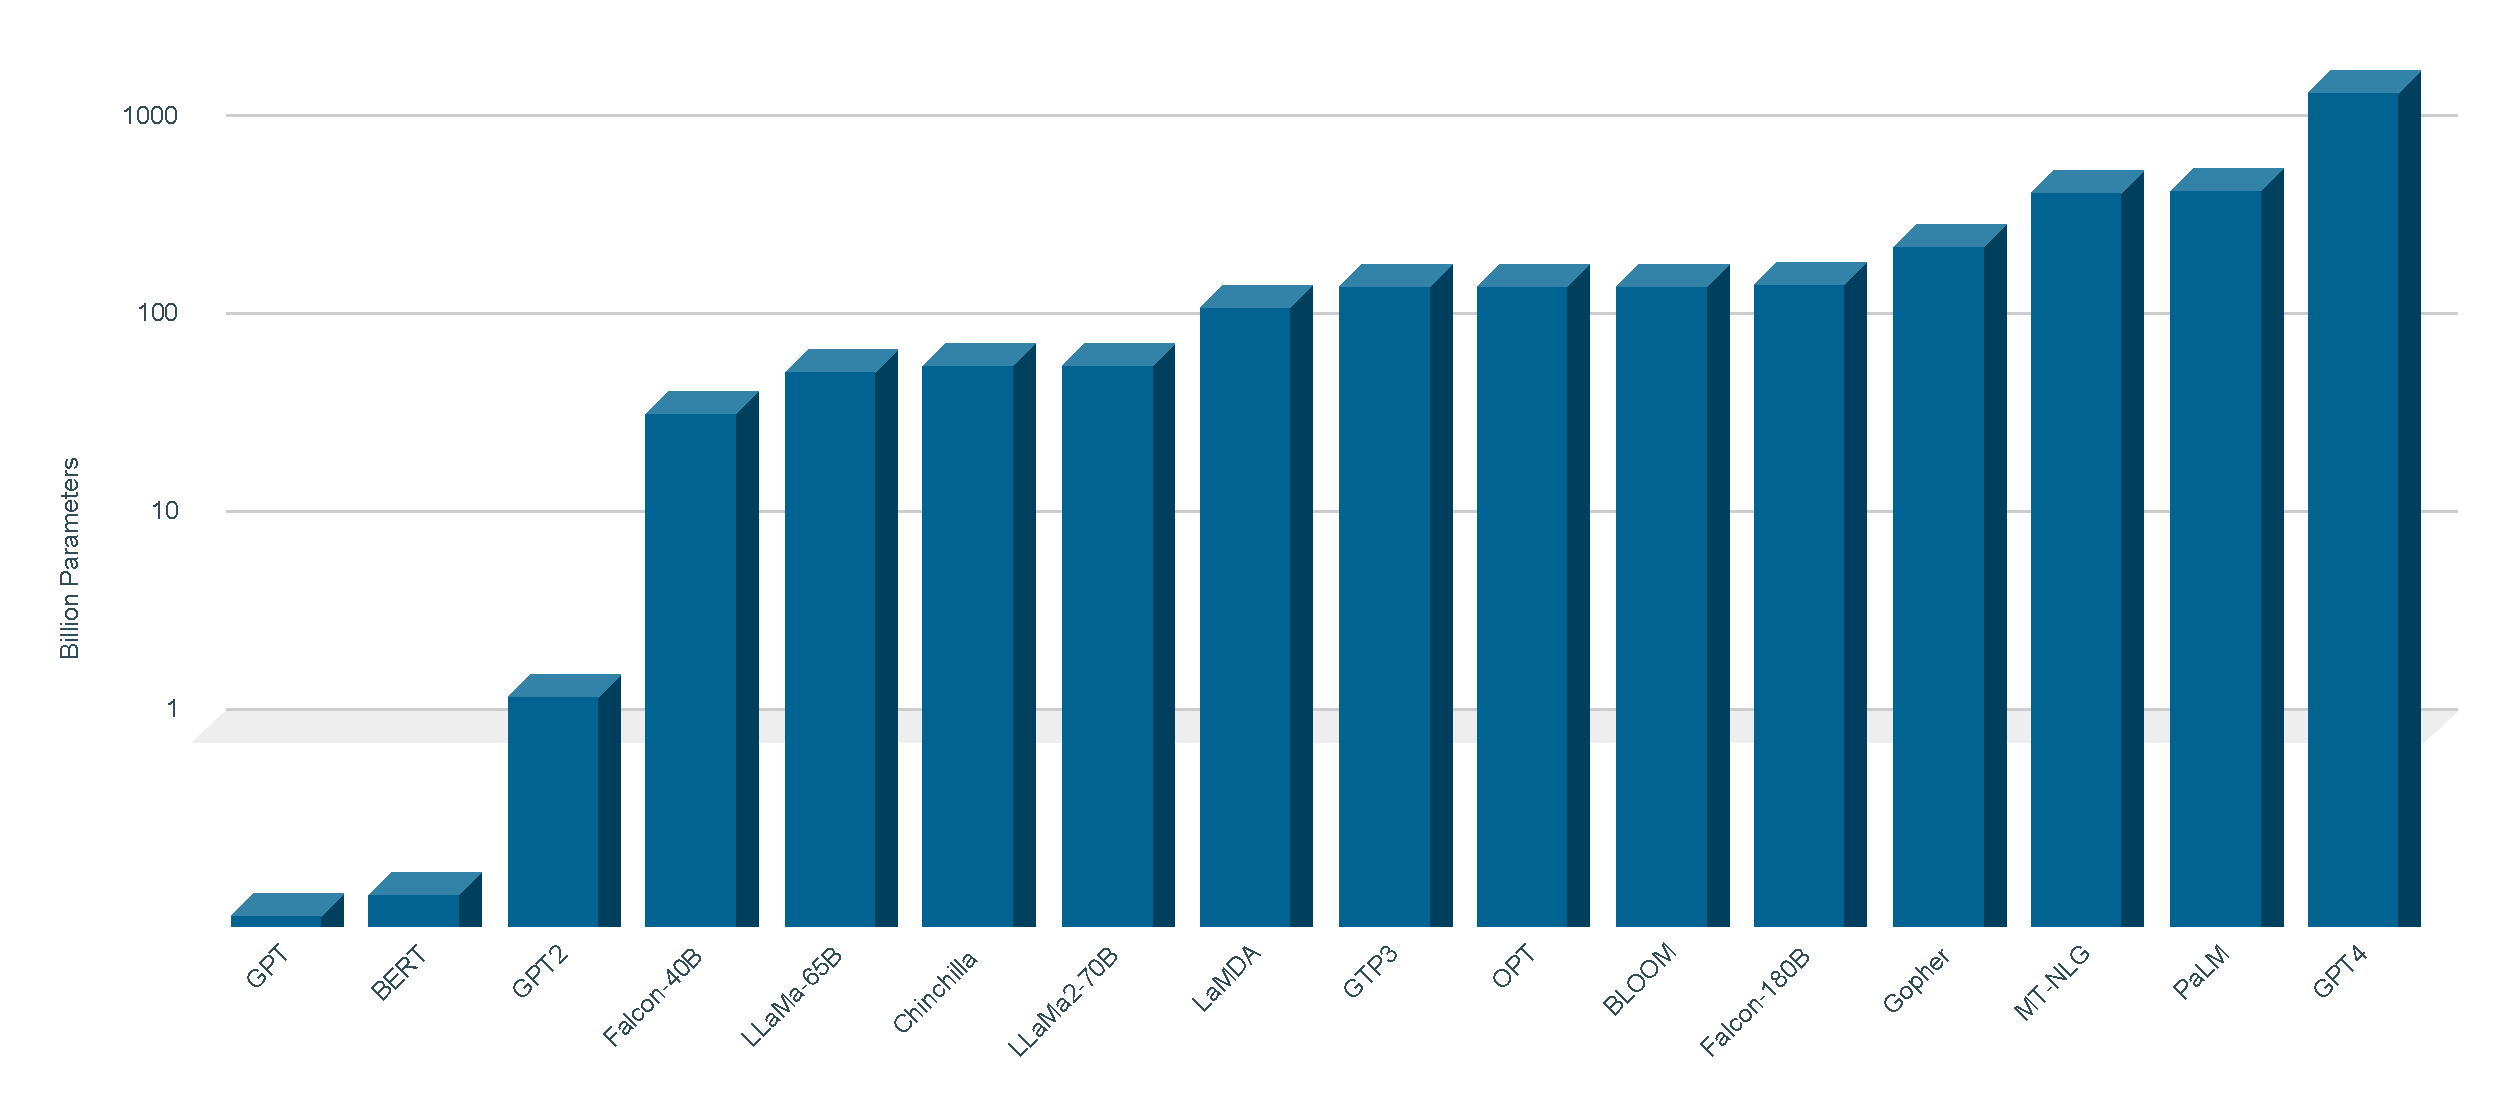
\includegraphics[height=0.7\textheight]{comparison_logscale}
\end{frame}


\begin{frame}[c]{Training Large Language Models}
    \begin{figure}
        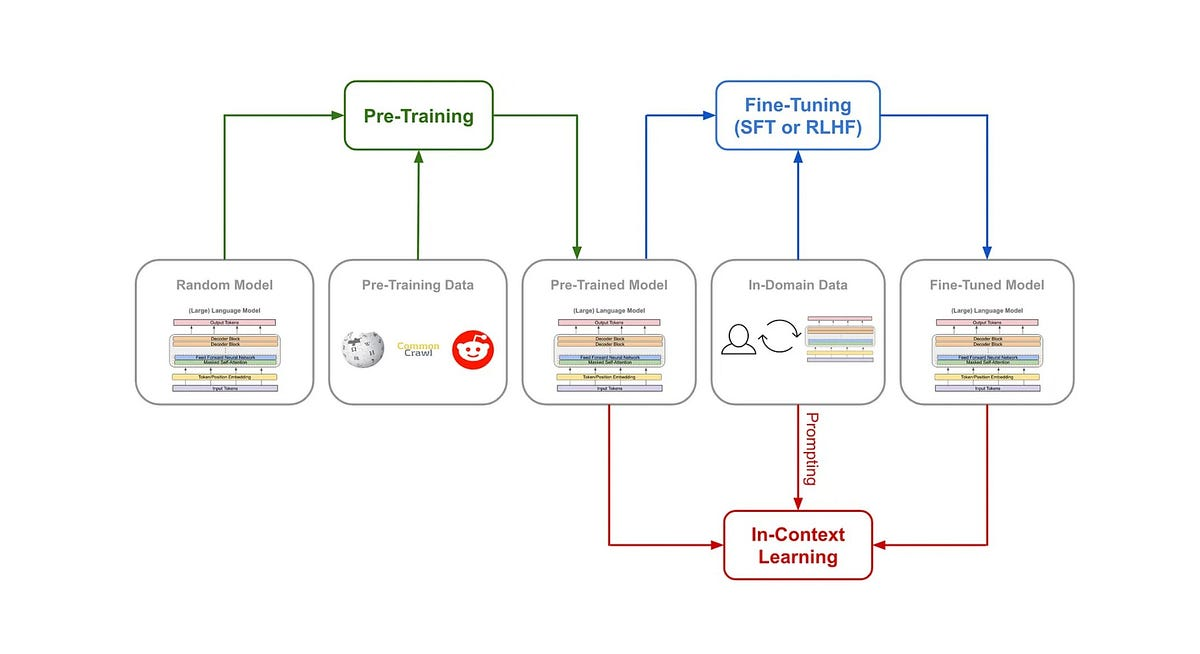
\includegraphics[height=0.65\textheight]{pre_training_fine_tuning}
        \caption{
            Image Source: \cite{ghosh_empowering_2023}
        }
    \end{figure}
\end{frame}
